Let $\omega_{m}$ with $m\in\inter{1}{M}$ be unit \emph{p}-vectors of unknown parameters.
The \tB{projection pursuit regression} (PPR):
\begin{center}
	\enc{$ f(X) = \su{{m=1}}{M}g_{m}(\omega_{m}^{T}X)$}
\end{center}
\sB{This is an additive model}, but in the derived features $V_{m}=\omega_{m}^{T}X$ rather than the
inputs themeselves.
\sB{The functions $g_{m}$ are unspecified and are estimated along with the directions $\omega_{m}$
using some flexible smoothing method.} The function $g_{m}(\omega_{m}^{T}X)$ is called a ridge
function in $\mathbb{R}^{p}$
The \sB{scalar variable $V_{m}=\omega_{m}X$ is the projection of $X$ onto the unit vector 
$\omega_{m}$} an we seek $\omega_{m}$ so that the model fits well, hence the name ``projection 
pursuit''.
\begin{figure}[H]
	\begin{center}
		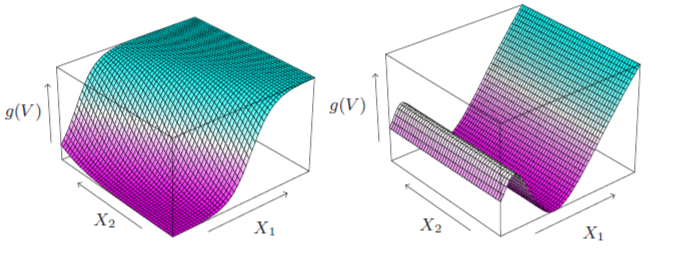
\includegraphics[width=\textwidth]{./chap/1chap/99sec/images/1_ridge_fct.PNG}
	\end{center}
	\caption{
	Perspective plots of 2 ridge functions.\\ Left: $g(V)=\dfrac{1}{1+e^{-5(V-0.5)}}$,
	where $V=\frac{X_{1}+X_{2}}{\sqrt(2)}$\\ Right: $g(V)=(V+0.1)\sin\left(\dfrac{1}{
	\frac{1}{3}+0.1}\right)$, where $V=X_{1}$}
	\label{fig:1_ridge_fct}
\end{figure}
We seek to approximate minimzers of the error function:
\begin{center}
	\encB{$ \su{{i=1}}{N}\left[y_{i}-\su{{m=1}}{M}g_{m}(\omega_{m}^{T}x_{i})\right]^{2}$}
\end{center}
over functions $g_{m}$ and direction vectors $\omega_{m}$.\\
Let $\omega_{old}$ be the current estimate for $\omega$.
$$ g(\omega^{T}x_{i})\approx g(\omega_{old}x_{i}) + g'(\omega_{old}^{T}x_{i})(\omega-
\omega_{old})^{T}x_{i}$$

\subsection{Neural Networks}
They are a large class of nonlinear statistical models much like the projection pursuit regression
model.\\
A neural network is a two-stage regression or classification model, represented by a network diagram:
\begin{figure}[H]
	\begin{center}
		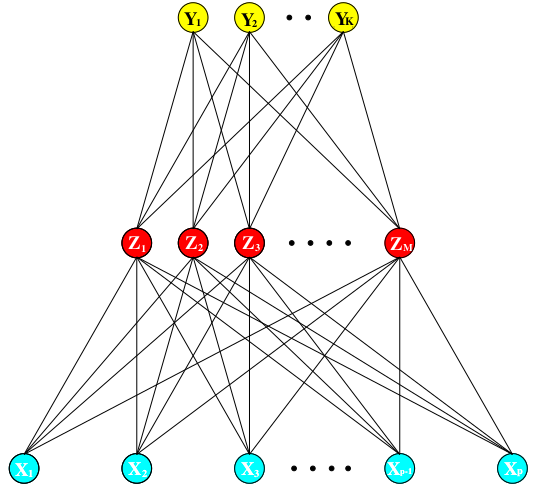
\includegraphics[width=.7\textwidth]{./chap/1chap/99sec/images/2_networkDiag.png}
	\end{center}
	\caption{Schematic of a single hidden layer, feed-forward neural network}
	\label{fig:99_2_networkDiag}
\end{figure}

For $K$-class classification, there are $K$ units at the top, with $k^{th}$ unit modeling the 
probability of class $k$. There are $K$ target measurements $\left\{Y_{k}:k\in\inter{1}{k}\right\}
\in {0, 1}^{K}$.\\
Derived features $Z_{m}$ are created from linear combinations of the $Z_{m}$:\\
$
\begin{cases}
	\forall m\in\inter{1}{M},~\bm{Z}_{m} = \sigma\left(\alpha_{0m}+\alpha_{m}^{T}\bm{X}\right)\\
	\forall k\in\inter{1}{K},~\bm{T}_{k} = \beta_{0k} + \beta_{k}^{T}\bm{Z}\\
	\forall k\in\inter{1}{K},~f_{k}(\bm{X}) = g_{k}(\bm{T})
\end{cases}
$\\
where 
$
Z =
\begin{pmatrix}
	Z_{1}\\
	\vdots\\
	Z_{M}
\end{pmatrix}
$ and 
$
T =
\begin{pmatrix}
	T_{1}\\
	\vdots\\
	T_{K}
\end{pmatrix}
$ 
The \tB{activation function} is usually chosen to be the sigmoid \encB{$\sigma(v) =
\dfrac{1}{1+e^{-v}}$}, the \tB{softmax} function is $g_{k}(T)=\dfrac{e^{T_{k}}}{\su{{l=1}}{K}e^{T_{l}}}$
